\documentclass[]{article}
\usepackage{lmodern}
\usepackage{amssymb,amsmath}
\usepackage{ifxetex,ifluatex}
\usepackage{fixltx2e} % provides \textsubscript
\ifnum 0\ifxetex 1\fi\ifluatex 1\fi=0 % if pdftex
  \usepackage[T1]{fontenc}
  \usepackage[utf8]{inputenc}
\else % if luatex or xelatex
  \ifxetex
    \usepackage{mathspec}
  \else
    \usepackage{fontspec}
  \fi
  \defaultfontfeatures{Ligatures=TeX,Scale=MatchLowercase}
\fi
% use upquote if available, for straight quotes in verbatim environments
\IfFileExists{upquote.sty}{\usepackage{upquote}}{}
% use microtype if available
\IfFileExists{microtype.sty}{%
\usepackage{microtype}
\UseMicrotypeSet[protrusion]{basicmath} % disable protrusion for tt fonts
}{}
\usepackage[margin=1in]{geometry}
\usepackage{hyperref}
\hypersetup{unicode=true,
            pdftitle={Towards the construction of a causal map of the human phenome},
            pdfauthor={Gibran Hemani, Jie Zheng, Philip Haycock, Oliver Davies, Jack Bowden, Tom Gaunt, George Davey Smith},
            pdfborder={0 0 0},
            breaklinks=true}
\urlstyle{same}  % don't use monospace font for urls
\usepackage{graphicx,grffile}
\makeatletter
\def\maxwidth{\ifdim\Gin@nat@width>\linewidth\linewidth\else\Gin@nat@width\fi}
\def\maxheight{\ifdim\Gin@nat@height>\textheight\textheight\else\Gin@nat@height\fi}
\makeatother
% Scale images if necessary, so that they will not overflow the page
% margins by default, and it is still possible to overwrite the defaults
% using explicit options in \includegraphics[width, height, ...]{}
\setkeys{Gin}{width=\maxwidth,height=\maxheight,keepaspectratio}
\IfFileExists{parskip.sty}{%
\usepackage{parskip}
}{% else
\setlength{\parindent}{0pt}
\setlength{\parskip}{6pt plus 2pt minus 1pt}
}
\setlength{\emergencystretch}{3em}  % prevent overfull lines
\providecommand{\tightlist}{%
  \setlength{\itemsep}{0pt}\setlength{\parskip}{0pt}}
\setcounter{secnumdepth}{0}
% Redefines (sub)paragraphs to behave more like sections
\ifx\paragraph\undefined\else
\let\oldparagraph\paragraph
\renewcommand{\paragraph}[1]{\oldparagraph{#1}\mbox{}}
\fi
\ifx\subparagraph\undefined\else
\let\oldsubparagraph\subparagraph
\renewcommand{\subparagraph}[1]{\oldsubparagraph{#1}\mbox{}}
\fi

%%% Use protect on footnotes to avoid problems with footnotes in titles
\let\rmarkdownfootnote\footnote%
\def\footnote{\protect\rmarkdownfootnote}

%%% Change title format to be more compact
\usepackage{titling}

% Create subtitle command for use in maketitle
\newcommand{\subtitle}[1]{
  \posttitle{
    \begin{center}\large#1\end{center}
    }
}

\setlength{\droptitle}{-2em}
  \title{Towards the construction of a causal map of the human phenome}
  \pretitle{\vspace{\droptitle}\centering\huge}
  \posttitle{\par}
  \author{Gibran Hemani, Jie Zheng, Philip Haycock, Oliver Davies, Jack Bowden,
Tom Gaunt, George Davey Smith}
  \preauthor{\centering\large\emph}
  \postauthor{\par}
  \predate{\centering\large\emph}
  \postdate{\par}
  \date{03 July 2017}

\usepackage{amsmath}

\begin{document}
\maketitle

\subsection{Abstract}\label{abstract}

A major application for genome-wide association studies (GWAS) has been
the emerging field of causal inference using Mendelian randomisation
(MR), where the causal effect between a pair of traits can be estimated
using only summary level data. MR depends on SNPs exhibiting vertical
pleiotropy, where the SNP influences an outcome phenotype only through
an exposure phenotype. Issues arise when this assumption is violated due
to SNPs exhibiting horizontal pleiotropy, and many methods have been
developed in an attempt to address this. Here we show that the
mechanisms that underlie horizontal pleiotropy are numerous, and that
instrument selection will be increasingly liable to selecting invalid
instruments as GWAS sample sizes continue to grow. We have developed a
mixture of experts machine learning approach (MR-MoE 1.0) that improves
on both power and false discovery rates over all existing methods. Using
the approach, we systematically estimated the causal effects amongst
2407 phenotypes, generating a draft of the causal map of the human
phenome. But we offer caution that its interpretation is far from
straightforward.

\subsection{Introduction}\label{introduction}

Mendelian randomisation (MR) (1,2) exploits genetic pleiotropy to infer
the causal relationships between phenotypes. Suppose that one trait (the
exposure) causally influences another (the outcome). If a SNP influences
the outcome through the exposure then the SNP is exhibiting vertical
pleiotropy. Such a genetic variant is considered to be an instrumental
variable for the exposure, and can be exploited to mimic a randomised
controlled trial, enabling a causal estimate to be made by comparing the
outcome phenotypes between those individuals that have the
exposure-increasing allele against those who do not. Multiple
independent genetic variants for a particular exposure can be used
jointly to improve causal inference, because a) each variant represents
an independent natural experiment, and an overall causal estimate can be
obtained by meta-analysing the single estimates from each instrument;
and b) some violations of the assumptions of MR (most notably that the
SNP influences the outcome through no pathways other than the exposure)
can be evaluated through sensitivity analyses (3--7).

Genome-wide association studies (GWAS) have identified genetic
instrumental variables for thousands of phenotypes (8). Recent
developments in Mendelian randomisation have enabled knowledge of
instrumental variables to be applied using only summary level data
(known as two-sample MR, 2SMR) (9). Here, in order to infer the causal
effect of an exposure on an outcome all that is required is an estimate
of the genetic effects of the instrumenting SNP on the exposure, and the
corresponding estimate of the effect on the outcome. This has two major
advantages. First, GWAS summary data is non-disclosive and often
publicly available. Second, causal inference can be made between
phenotypes even if they have not been measured in the same samples,
limiting the breadth of possible causal estimates only to the
availability of GWAS summary data for the traits in question (10).

Problems with obtaining unbiased causal effects can arise, however, if
the genetic instruments exhibit horizontal pleiotropy (HP), where they
influence the outcome through a pathway other than the exposure. The
extent of this phenomenon is not to be understated, and many methods
have been developed that attempt to reliably obtain unbiased causal
estimates under specific models of HP (3--6). It is considered best
practice to report estimates from all available methods as sensitivity
analyses when presenting causal estimates, however this strategy is not
necessarily optimal for several reasons. First, if different methods
disagree it is not possible to know which is correct because the true
nature of HP exhibited by the instruments is not known. Second, though
the IVW approach is most statistically powerful under no HP, it can have
high false negative or low true positive rates in the presence of HP
compared to other methods. Given that pleiotropy has been hypothesised
to be universal (11,12), defaulting to the IVW method in the first
instance and using other methods as sensitivity analyses may not be
appropriate. Third, the available methods do not cover all possible
models of HP, and therefore an automated method for instrument selection
may be necessary. Fourth, it could be of interest to make causal effect
estimates for thousands of traits, in which case a discerning evaluation
of each causal effect of interest may not be possible or convenient.

In this paper we introduce two innovations towards improving the
reliability of MR estimates. First, we introduce an approach to discard
genetic variants that are likely to be invalid. Second, we hypothesised
that characteristics of the summary data could indicate which method
would be most reliable, and we introduce new machine learning approaches
that attempt to automate both instrument and method selection. Using
curated GWAS summary data for thousands of phenotypes (10), we use these
new methods to construct a graph of millions of causal estimates. We
consider this to be a `first draft' of the causal map of the human
phenome, but raise caution throughout that its interpretation is far
from straightforward

\subsection{Methods}\label{methods}

\subsubsection{GWAS summary data and their use in
2SMR}\label{gwas-summary-data-and-their-use-in-2smr}

The use of summary data in two-sample MR is described in detail
elsewhere (10). A brief outline of the procedure is as follows. First,
genetic instruments for the exposure trait need to be identified - those
SNPs with \(p < 10^{-8}\) are retained in order to ensure that the first
assumption of Mendelian randomisation (that the instrument associates
with the exposure) is satisfied. We collect their effect sizes, standard
errors and effect alleles for the association with the exposure trait.
These can be obtanied manually from complete summary data or from
curated lists of significant GWAS associations. Next, the effects of
those SNPs on the outcome need to be obtained, typically necessitating
complete summary data because it is unlikely that these SNPs will have
reached genome-wide significance (and therefore be present in curated
catalogues). At its most simple implementation, the regression of the
SNP-exposure effect sizes against the SNP-outcome effect sizes, with
greater weight afforded to those SNPs with smaller SNP-outcome standard
errors, provides the estimate of the causal effect of the exposure on
the outcome. This is known as the inverse-variance weighted (IVW)
method.

Given summary data for a large number of traits, it is straightforward
to exhaustively analyse the causal relationships of every trait against
every other trait for which there is sufficient summary data available.
Supplementary table 1 provides a list of all traits that have available
GWAS summary data, indicating if they have complete summary data (in
which case they can be used as both exposure traits and outcome traits),
or if they only have significant associations (in which they can only be
used as exposure traits).

\subsubsection{Mendelian randomisation methods and their
assumptions}\label{mendelian-randomisation-methods-and-their-assumptions}

In this paper we consider three main classes of MR estimation. Full
details for each approach have been described extensively elsewhere.

\textbf{Mean-based methods:} Here we consider four nested models (5).
The inverse variance weighted (IVW) fixed effects meta-analysis approach
assumes that variants exhibit no HP. IVW random effects meta-analysis
relaxes the HP assumption, allowing it to be present but balanced - such
that it only leads to increased heterogeneity around the regression and
not introducing bias. Fixed effects Egger regression (3) relaxes the HP
assumption further by allowing a non-zero intercept which essentially
allows horizontal pleiotropy to be directional, where it systematically
influences the outcome in a specific direction. Random effects Egger
regression allows heterogeneity around the directional HP, as long as
the HP effects are not correlated with the SNP-exposure effects (also
known as the INSIDE assumption).

The Rucker framework (13), adapted to MR (5) uses estimates of
heterogeneity in the IVW and Egger frameworks to navigate between these
nested models. A jackknife approach (random selection with replacement
of instruments) can be used to obtain a sampling distribution for the
model estimate amongst these four variations. Using 1000 rounds of
jackknife estimates, we can obtain a final estimate using the mean or
the median of the distribution. We only use the jackknife approach for
associations where there are 15 or more variants to avoid combinatorial
saturation. The four nested models plus the three Rucker estimates
provide seven mean based estimators.

\textbf{Median-based methods:} An alternative approach is to take the
median effect of all available instruments (4). This has the advantage
that up to half the instruments can be invalid, and the estimate will
remain unbiased. Developing the approach further to allow stronger
instruments to contribute more towards the estimate can be obtained by
obtaining the median of the weights of each instrument. The penalised
weighted median estimator introduces a further weight to the
instruments, penalising any instrument that contributes substantially
towards the heterogeneity statistic. Together, this provides three
median based estimators.

\textbf{Mode-based methods:} Similar to the median, the mode based
estimator clusters the instruments into groups based on similarity of
causal effects, and returns the final causal effect estimate based on
the cluster that has the largest number of instruments (6). This can be
extended in two ways, first by weighting the strength of each cluster by
the inverse of the variance of the SNP-outcome associations in the
cluster; second by weighting the strength of each cluster by the inverse
of the variance of the SNP-exposure associations. When weighting by the
SNP-outcome standard errors we term this a weighted analysis. When
\emph{not} weighting by the exposure standard errors we term this the
`no measuremenent error in the exposure (NOME)' assumption. Together
this provides four mode-based estimators.

\subsubsection{Instrument selection}\label{instrument-selection}

\paragraph{Top hits}\label{top-hits}

The simplest approach to selecting instruments for performing MR is to
take take SNPs that have been declared significant in the published GWAS
for the exposure. This typically involves obtaining SNPs that surpass
\(p < 5 \times 10^{-8}\), using clumping to obtain independent SNPs, and
then replicating in an independent sample. These results are often
recorded in public GWAS catalogs. Alternatively the clumping procedure
can be performed using complete summary data in MR-Base. We call this
the ``top hits'' strategy.

\paragraph{Steiger filtering}\label{steiger-filtering}

With genome-wide association studies growing ever larger, the
statistical power to detect significant associations that may be
influencing the trait downstream of many other pathways increases. For
example, if a SNP \(g_{A}\) influences trait \(A\), and trait \(A\)
influences trait \(B\), then a sufficiently powered GWAS will identify
the \(g_{A}\) as being significant for trait \(B\) (Figure 1a). Using
\(g_{A}\) as an instrument to test the causal effect of \(A\) on \(B\)
is perfectly valid. But in the (incorrectly hypothesised) MR analysis of
trait \(B\) on trait \(A\) could erroneously result in the apparent
causal association of \(B\) on \(A\). If \(g_{A}\) is only one of many
known instruments for \(B\), amongst which some are valid, it is to the
advantage of the researcher to exclude \(g_{A}\) from the analysis.

An approach to inferring the causal direction between phenotypes was
developed recently (7), using the following basic premise. If trait
\(A\) causes trait \(B\) then

\[
\sum^M_{i=1}{cor(g_{i}, A)^2} > \sum^M_{i=1}{cor(g_{i}, B)^2}
\]

because the \(cor(g_{i}, B)^2 = cor(A, B)^{2} cor(g_{i}, A)^{2}\). This
simple inequality will not hold in some cases, for example
\(\rho_{x, x_o} < \rho_{x,y}\rho_{y,y_o}\) where \(\rho_{x, x_o}\) and
\(\rho_{y, y_o}\) are the precision of the measurements of the \(x\) and
\(y\). Some combinations of confounding effects can also distort the
\(\rho_{g,x}\) and \(\rho_{g,y}\) parameters, as has been discussed in
detail previously. However, we use it here as an inexpensive and
approximate method to identify variants that are likely to be invalid.
Steiger's Z-test of correlated correlations (14) can be used to formally
test the extent to which the two correlations are statistically
different.

Here we adapt this approach to automatically filter SNPs that are liable
to be invalid (Figure 1a). In this case the Steiger test applied to each
variant in turn and we exclude any \(g_{A}\) for which the Steiger
Z-test has \(p > 0.05\), indicating that it is unlikely to primarily
associate with \(B\) relative to \(A\). Similarly, for SNPs that
influence confounders of \(A\) and \(B\) or those variants that exhibit
horizontal pleiotropy, the difference in \(cor(g_{i}, A)^2\) and
\(cor(g_{i}, B)^2\) will be reduced, increasing the likelihood of the
SNP being excluded because the Steiger Z-test is less likely to be
significant.

To estimate \(cor(g, x)^2\), if \(x\) is continuous we obtain the
F-statistic from the reported p-value and sample size and then
\(cor(g, x)^2 = \frac{F}{N - 2 - F}\). If \(x\) is binary then we
estimate the variance of the underlying liability explained by the SNP,
\(cor(g, x)^2 = \frac{V_a}{V_a + V_e}\). Here, \(V_e = \pi^2/3\), and
\(V_a = 2\beta^2p(1-p)\), where \(\beta\) is the log odds ratio and
\(p\) is the allele frequency of the SNP in the population (15). \(p\)
can be estimated using the allele frequency of the SNP in an ascertained
sample by deriving the \(2 \times 2\) contingency table from the odds
ratio \(e^\beta\), allele frequency in the ascertained sample
\$p\_\{cc\}, and number of cases \(N_1\) and controls \(N_0\).

\subsubsection{Competitive mixture of
experts}\label{competitive-mixture-of-experts}

We consider the 14 MR methods described above, for which instruments can
be supplied using two instrument selection strategies, leading to 28
methods in total. In the context of this analysis, each method is
considered to be an `expert', taking a set of SNP-exposure and
SNP-outcome effect sizes and their standard errors as inputs. Our
objective is to select the expert most likely to be correct for a
specific MR analysis.

The mixture of experts method is a machine learning approach (16) which
seeks to divide a parameter space into subdomains, such that a
particular expert is used primarily for problems that reside in a
subdomain most suited to that expert. In this case our objective is to
identify characteristics of the SNP-exposure and SNP-outcome
associations for which one specific MR method is most likely to yield
highest statistical power for non-null associations, and lowest false
discovery rates for null associations. This involves creating a `gating
function', whose purpose is to decide which expert to use for a specific
MR analysis, given the parameter space that is occupied by that dataset.
The metrics are a mixture of regression diagnostics and are described in
Supplementary table 2.

The gating function needs to be trained using data for which the true
causal effect is known, and to this end we generated a large number of
simulated datasets. We trained the gating function using random forest
learning algorithms that seek to identify sectors of the parameter space
that are most likely to return accurate estimates for a particular
expert. Figure 2a illustrates how the gating function is trained using
simulated data. New datasets can then be applied to the trained mixture
of experts (MoE) model (Figure 2b). There are countless ways to
implement this approach, we call this implementation MR-MoE 1.0.

\textbf{Training and testing simulations}

The MoE is trained using datasets generated from simulations (Figure
2a). A \emph{dataset} is the minimum data required to perform 2SMR
analysis - four columns comprising the SNP-exposure and SNP-outcome
effects and standard errors, and rows corresponding to each SNP that is
used as an instrument for the exposure. This \emph{dataset} can be fed
into any of the 28 experts to obtain MR causal effects. The simulations
used to generate these datasets seek to cover a range of pleiotropic
scenarios, including where some proportion of SNPs exhibit directional
or balanced horizontal pleiotropy, or where SNPs influencing confounding
variables.

We simulate two individual level datasets for which there are \(N_x\)
and \(N_y\) samples, and \(M\) SNPs, where each SNP has effect allele
frequency of \(p_m \sim U(0.05, 0.95)\). These datasets are used to
obtain the SNP effects for the exposure trait \(x\) and the outcome
trait \(y\), respectively, using the following sampling criteria:

\[
\begin{aligned}
N_x & = \{20000, ..., 500000\} \\
N_y & = \{20000, ..., 500000\} \\
K & = \{0, ..., 10\} \\
M_x & = \{1, ..., 200\} \\
M_y & = \{1, ..., 200\} \\
M_{u_k} & = \{5,..., 30\} \\
\end{aligned}
\]

The \(M = M_x + M_y + \sum{M_{u_k}}\) SNPs can influence \(x\) directly,
\(y\) directly, or some number of confounders \(u_{k}\) directly.
Phenotypes for \(x\) and \(y\) are constructed using

\[
x = \sum^{M_x}_{i}{\beta_{gx,x,i}g_{x,i}} + \sum^{M_y}_{j}{\beta_{gy,x,j}g_{y,j}} + \sum^{K}_{k}{\beta_{ux,k} u_{k}} + e_{x}
\]

where \(\beta_{gx,x}\) is the vector of effects of each of the \(M_x\)
SNPs that influence \(x\) primarily, \(\beta_{gy,x}\) is the vector of
effects for the \(M_y\) SNPs on \(x\), where the \(M_y\) SNPs influence
\(y\) primarily but exhibit horizontal pleiotropic effects on \(x\). We
allow some proportion of these effects to be 0. \(\beta_{ux}\) is the
vector of effects of each of the \(K\) confounders on \(x\). Each
\(u_{k}\) variable is constructed using

\[
u = \sum^{M_u}_{l}{\beta_{gu,l}g_{l}} + e_{l}
\]

and finally \(y\) is constructed using

\[
y = \beta_{x,y}x + \sum^{M_y}_{i}{\beta_{gy,y,j}g_{y,j}} + \sum^{M_x}_{j}{\beta_{gx,y,i}g_{x,i}} + \sum^{K}_{k}{\beta_{uy,k} u_{k}} + e_{y}
\]

where \(\beta_{x,y}\) is the causal effect of \(x\) on \(y\). We sample
the distribution of direct SNP effects using

\[
\begin{aligned}
\beta_{gx,x,i} & \sim N(0, \sigma^2_{gx,x}) \\
\sigma^2_{gx,x,i} & \sim U(0.01, 0.1) \\
\beta_{gy,y,j} ~ N(0, \sigma^2_{gy,y}) \\
\sigma^2_{gy,y,j} & \sim U(0.01, 0.1) \\
\end{aligned}
\]

Some proportion \(s_x \sim U(0,1)\) of \(g_x\) SNPs and some proportion
\(s_y \sim U(0,1)\) of \(g_y\) SNPs exhibit horizontal pleiotropy with
effects sampled using

\[
\begin{aligned}
\beta_{gx,y,i*} & \sim N(\mu_{gx,y}, \sigma^2_{gx,y})  \\
\mu_{gx,y,i*} & \sim U(-0.005, 0.005) \\
\sigma^2_{gx,y,i*} & \sim U(0.001, 0.01) \\
\beta_{gy,x,j*} & \sim N(\mu_{gy,x}, \sigma^2_{gy,x}) \\
\mu_{gy,x,j*} & \sim U(-0.005, 0.005) \\
\sigma^2_{gy,x,j*} & \sim U(0.001, 0.01) \\
\end{aligned}
\]

The genetic influences on each of the confounders are sampled using

\[
\begin{aligned}
\beta_{gu,u,l} & \sim N(0, \sigma^2_{gu,u}) \\
\sigma^2_{gu,u,l} & \sim U(0.01, 0.1) \\
\end{aligned}
\]

The influence of each confounder on \(x\) and \(y\) is obtained using

\[
\begin{aligned}
\beta_{u,x} & \sim N(0, \sigma^{2}_{u,x}) \\
\beta_{u,y} & \sim N(0, \sigma^{2}_{u,y}) \\
\end{aligned}
\]

Finally, 20\% of the simulations have a null effect of
\(\beta_{x,y} = 0\), while the other remaining 80\% have a true effect
sampled from

\[
\begin{aligned}.
\beta_{x,y} & \sim N(0, \sigma^2_{x,y}) \\
\sigma^2_{x,y} & \sim U(0.001, 0.1) \\
\end{aligned}
\]

For each simulation we used linear regression to estimate the genetic
effect of each SNP \(M\) on \(x\) in sample 1, and each SNP \(M\) on
\(y\) in sample 2. We then perform MR analysis in both directions,
retaining SNPs that have \(p < 5e-8\) in sample 1 to perform MR of \(x\)
on \(y\) (the true causal direction for non-null simulations), and
retaining SNPs that have \(p < 5e-8\) in sample 2 to perform MR of \(y\)
on \(x\) (the reverse causal direction for non-null simulations). We
treat the summary data (effect sizes and standard errors) used for
estimating \(x \rightarrow y\) the summary data used for estimating
\(y \rightarrow x\) as two separate datasets Hence, for each simulation
two datasets are generated which are analysed to produce 28 MR estimates
each. We performed 100,000 simulations using these parameters, resulting
in 200,000 datasets.

\textbf{Optimisation function}

We aim to maximise statistical power for datasets where
\(\beta_{x,y} \neq 0\) and minimise false discovery rates for datasets
where \(\beta_{x,y} = 0\). To train random forest decision trees to
predict performance for a particular method
\(h(O_{w,d}, \textbf{z}_{d}\) is generated where the training set of
input metrics for dataset \(d\) is \(\textbf{z}_{d}\) and the response
(optimisation function) is

\[
    O_{w,d} = 
\begin{cases}
    1,   & \text{if } \beta_{x,y} \neq 0 \text{and } p_{m,d} < 0.01\\
    1,   & \text{if } \beta_{x,y} = 0 \text{and } p_{m,d} > 0.1 \\
    0,   & \text{otherwise}
\end{cases}
\]

\textbf{Strategy}

For each training dataset we record a set of 53 metrics
\(\textbf{z}_{d}\) (Supplementary table 2), and an outcome \(O_{w,d}\),
which is a measure of how well that method performed for each particular
simulated dataset. For each of our 28 methods, we need to create a model
that predicts the performance of the method based on metrics generated
from a dataset. To do this, for each method we train random forest
decision trees to predict that method's performance using the dataset's
metrics. The random forest approach is well suited to this problem
because there are likely to be non-continuous combinations of different
metrics that improve on prediction over, for example, a simple linear
model that does not learn about interactions.

A simple hypothetical example - if a dataset has a single outlier but is
otherwise exhibiting no heterogeneity then the following methods could
arguably perform well:

\begin{itemize}
\tightlist
\item
  an IVW fixed effects analysis with the outlier removed, should the
  Steiger test be able to detect the outlier
\item
  a median based approach
\item
  a mode based approach
\end{itemize}

deciding between these methods requires finding, in general, which will
minimise false discovery rates and maximise true positive rates for that
particular scenario.

Having generated random forest decision trees for each of the 28 methods
using 133,000 of the simulations, we then applied them to the remaining
67,000 datasets to predict which method would have the highest
performance for each of the remaining datasets. Finally we compare the
performance of the method selected by the MoE against all remaining
methods. The default settings for the \texttt{randomForest} package in R
(17) was used to train the models. MR-MoE 1.0 is implemented in the
TwoSampleMR R package available at
\href{https://github.com/MRCIEU/TwoSampleMR}{github.com/MRCIEU/TwoSampleMR}.

\subsubsection{Graph database of MR
estimates}\label{graph-database-of-mr-estimates}

The set of MR estimates obtained from this analysis are recorded in a
Neo4j graph database. Because each association has up to 28 different
estimates, for simplicity we distill this down to a single `best
estimate' for each association using the following rules:

\begin{enumerate}
\def\labelenumi{\arabic{enumi}.}
\tightlist
\item
  If the number of variants after Steiger filtering is greater than 5
  then apply the MoE to obtain the best method
\item
  If the number of variants after Steiger filtering is less than or
  equal to 5 but greater than 1 then use the IVW random effects approach
  on the filtered set of variants
\item
  If there is 1 variant retained in the Steiger approach then use the
  Wald ratio on the remaining variant
\item
  If there are no variants remaining after Steiger filtering then
  declare no causal association.
\end{enumerate}

For specific hypotheses we strongly recommend that estimates from all
sensitivity analyses are scrutinised and reported. The graph can be
queried directly using the cypher language at
\url{http://shark.epi.bris.ac.uk:7474/browser/} or through a basic web
interface at \url{http://shark.epi.bris.ac.uk:3838}.

\subsection{Results}\label{results}

\subsubsection{Steiger filtering improves
reliability}\label{steiger-filtering-improves-reliability}

As statistical power for GWAS studies improves the likelihood of a
significant association being discovered that doesn't act primarily on
the trait of interest increases (Figure 1a). We evaluated the efficacy
of the Steiger filtering approach for improving instrument selection
using 100,000 simulated datasets comprising both null and non-null
causal models. For each dataset, instruments were selected based on the
tophits strategy and the Steiger filtering strategy, and MR was
performed using 14 different methods based on instruments selected from
each of these strategies.

Figure 1b shows that the tophits strategy led to 49\% of the instruments
being primarily associated with either confounders or the outcome
phenotype, not the exposure phenotype. Applying Steiger filtering
reduced this to 25\%. Consequently, the false discovery rates (FDR) for
12 of the 14 methods reduced substantially when applied using Steiger
filtered instruments (Figure 1c). The true positive rates for the
methods based on Steiger filtering did however reduce slightly for 10 of
the 14 methods.

\subsubsection{Mixture of experts method selection improves over any
single
method}\label{mixture-of-experts-method-selection-improves-over-any-single-method}

Following evidence that the Steiger filtering approach can improve on
existing methods, we next hypothesised that a mixture of experts (MoE)
model would be able to use dataset characteristics to predict the most
appropriate of the 28 MR methods and instrument selection strategies
(Figure 2).

The ability to predict the performance for each of these methods is
shown in table 1, with prediction \(R^2\) ranging between 0.04 and 0.24.
The dataset characteristics with the most importance for each of the
predictors differed substantially between each dataset, as well as the
frequency for which each of the methods was selected in the testing
datasets. The FDR of each method when chosen, compared to their averages
across all datasets, reduced; and likewise the true positive rates of
each method when chosen increased compared to their simulation-wide
averages.

We compared the MoE performance in the simulations against each of the
28 methods, testing to see if it outperformed all other single methods.
Figures 3a and 3b show that the MoE approach had the best general
performance, obtaining an AUC of 0.84 in terms of classifying the
simulations as being null or non-null. Notably, the next best methods
were median and mode based estimators using Steiger filtering. Under the
assumption of universal pleiotropy it is clear that all methods suffer
from high false discovery rates.

\subsubsection{Automated MR analysis of 2407
phenotypes}\label{automated-mr-analysis-of-2407-phenotypes}

We applied our analysis using summary data for 2407 phenotypes,
including 149 complex traits and diseases, 575 metabolites (18,19) and
1683 plasma protein levels (20). For the protein levels only the
instruments were available, so they could only be evaluated as exposure
phenotypes. The complex traits and diseases and metabolite levels had
complete summary data available in MR-Base, thus they be evaluated as
both exposures (if they had significant instruments) and outcomes.
Together, we evaluated 715681 relationships. The majority of these
associations could only be evaluated using fewer than 5 SNPs, and so the
Wald ratio or IVW fixed effects methods were used, but for 61029
associations the MR-MoE approach was applied.

There were 5660 associations following Bonferroni correction
(\(p < 7.0\times^{-8}\)). Of these 2918 were obtained from the MR-MoE
analysis, while the remainder were estimated using fewer than 5 SNPs
using the Wald ratio or IVW fixed effects methods.

The frequencies of the methods chosen by the MR-MoE analysis are shown
in Supplementary table 2. Amongst those deemed `significant', the IVW
fixed effects analysis using tophits instruments (the only method
applicable when there is no evidence of horizontal pleiotropy of any
sort) was selected in only 10.4\% of cases.

\subsubsection{Causal associations involving years of
schooling}\label{causal-associations-involving-years-of-schooling}

As an example of the database, we performed a look up of associations
that causally influence years of schooling (21), or that years of
schooling itself causally influences. Using a false-discovery rate of
0.05, 45 traits were returned as having some direction of causality with
years of schooling (Figure 4). Though many of these putative
relationships appear to be plausible, it is clear that there are serious
limitations to using MR as a panacea for causal inference. For example,
bi-directional causal relationships with college completion exist
because of the similarity in trait definitions; and there are several
traits (e.g.~childhood intelligence and birth weight) which appear to be
causally downstream of years of schooling despite this being temporally
impossible. The facility to perform these scans has been automated at
the MR of everything vs everything (MR-EvE) website,
\url{http://shark.epi.bris.ac.uk:3838}, though we urge caution on
interpretation of these findings.

\subsection{Discussion}\label{discussion}

Following a recent flurry in development of MR methodology, we have
devised a machine learning approach, MR-MoE, that seeks to predict the
performance of each MR method, selecting the one which is most likely to
maximise power whilst minimising FDR for a specific dataset. The mixture
of experts approach that we present here is trained using random forest
decision trees applied to extensive and diverse simulations, and we
demonstrate that it makes substantial performance improvements over any
other single method.

Crucially, we observed in our simulations that none of the available
methods were conservative and all, including MR-MoE, had FDR above 0.2.
Instrumental variables in Mendelian randomisation are typically chosen
blind, with GWAS significance being the only criteria. We illustrated
how confounders and reverse causal associations can easily lead to
invalid instruments being used in MR, and that even if those instruments
that only influence the exposure directly, most randomly generated
patterns of horizontal pleiotropy cannot be adequately accounted for by
any single MR method.

We applied the method to a curated set of GWAS summary data that was
present in MR-Base (22), generating hundreds of thousands of MR
estimates. MR-MoE selected a method that indicated some pattern of
horizontal pleiotropy for almost 90\% of cases, suggesting that it is
the rule rather than the exception. Based on our simulations we expect
that those associations that we reported to be `significant' are liable
to high type 1 error rates.

In addition to correctly handling horizontal pleiotropy, there are many
other limitations that prevent MR from being a panacea for causal
inference. Many of the associations are biologically impossible, for
example where early life phenotypes appear to be influenced by later
stage phenotypes. Though these associations can be informative, their
interpretations as causal relationships are far from clear. Similarly,
often disease traits appear to causally relate to other phenotypes, but
GWAS is typically performed on the liability scale, hence the causal
estimate reflects not the presence or absence of disease, but the
underlying risk of disease. Again, interpretation of such associations
can be problematic.

A large proportion of the associations that were estimated used only a
single instrumental variable. Methods are emerging to attempt to
delineate between models of reverse cause, pleiotropy and multiple
causal variants in the same region (23,24), but separating vertical from
horizontal pleiotropy with a single instrument is not yet possible in
the two-sample MR framework. Other problems can also manifest, for
example frailty effects could induce associations for late-onset traits
(25). We also encounter a potential new problem when it comes to using
machine learning approaches to infer the correct model for a particular
dataset, namely, that the data is choosing the model. This is liable to
increase type 1 error rates, even though we have attempted to separate
the information used for optimisation from the information used to
predict performance. Though MR-MoE has high type 1 error rates, they
still remain amongst the lowest compared to all other methods that do
not suffer from this issue.

Despite these limitations, the construction of a causal graph of
`everything versus everything' does have appeal. First, though causality
is not guaranteed by MR, it can still be highly informative for
confirming or negating specific hypotheses, or to search for novel
putative associations. The potential to exploit GWAS summary data within
the properties of graph databases to aid with both of these endeavours
could be transformative in biological research.

\subsection{Figures}\label{figures}

\newpage

\begin{figure}
\centering
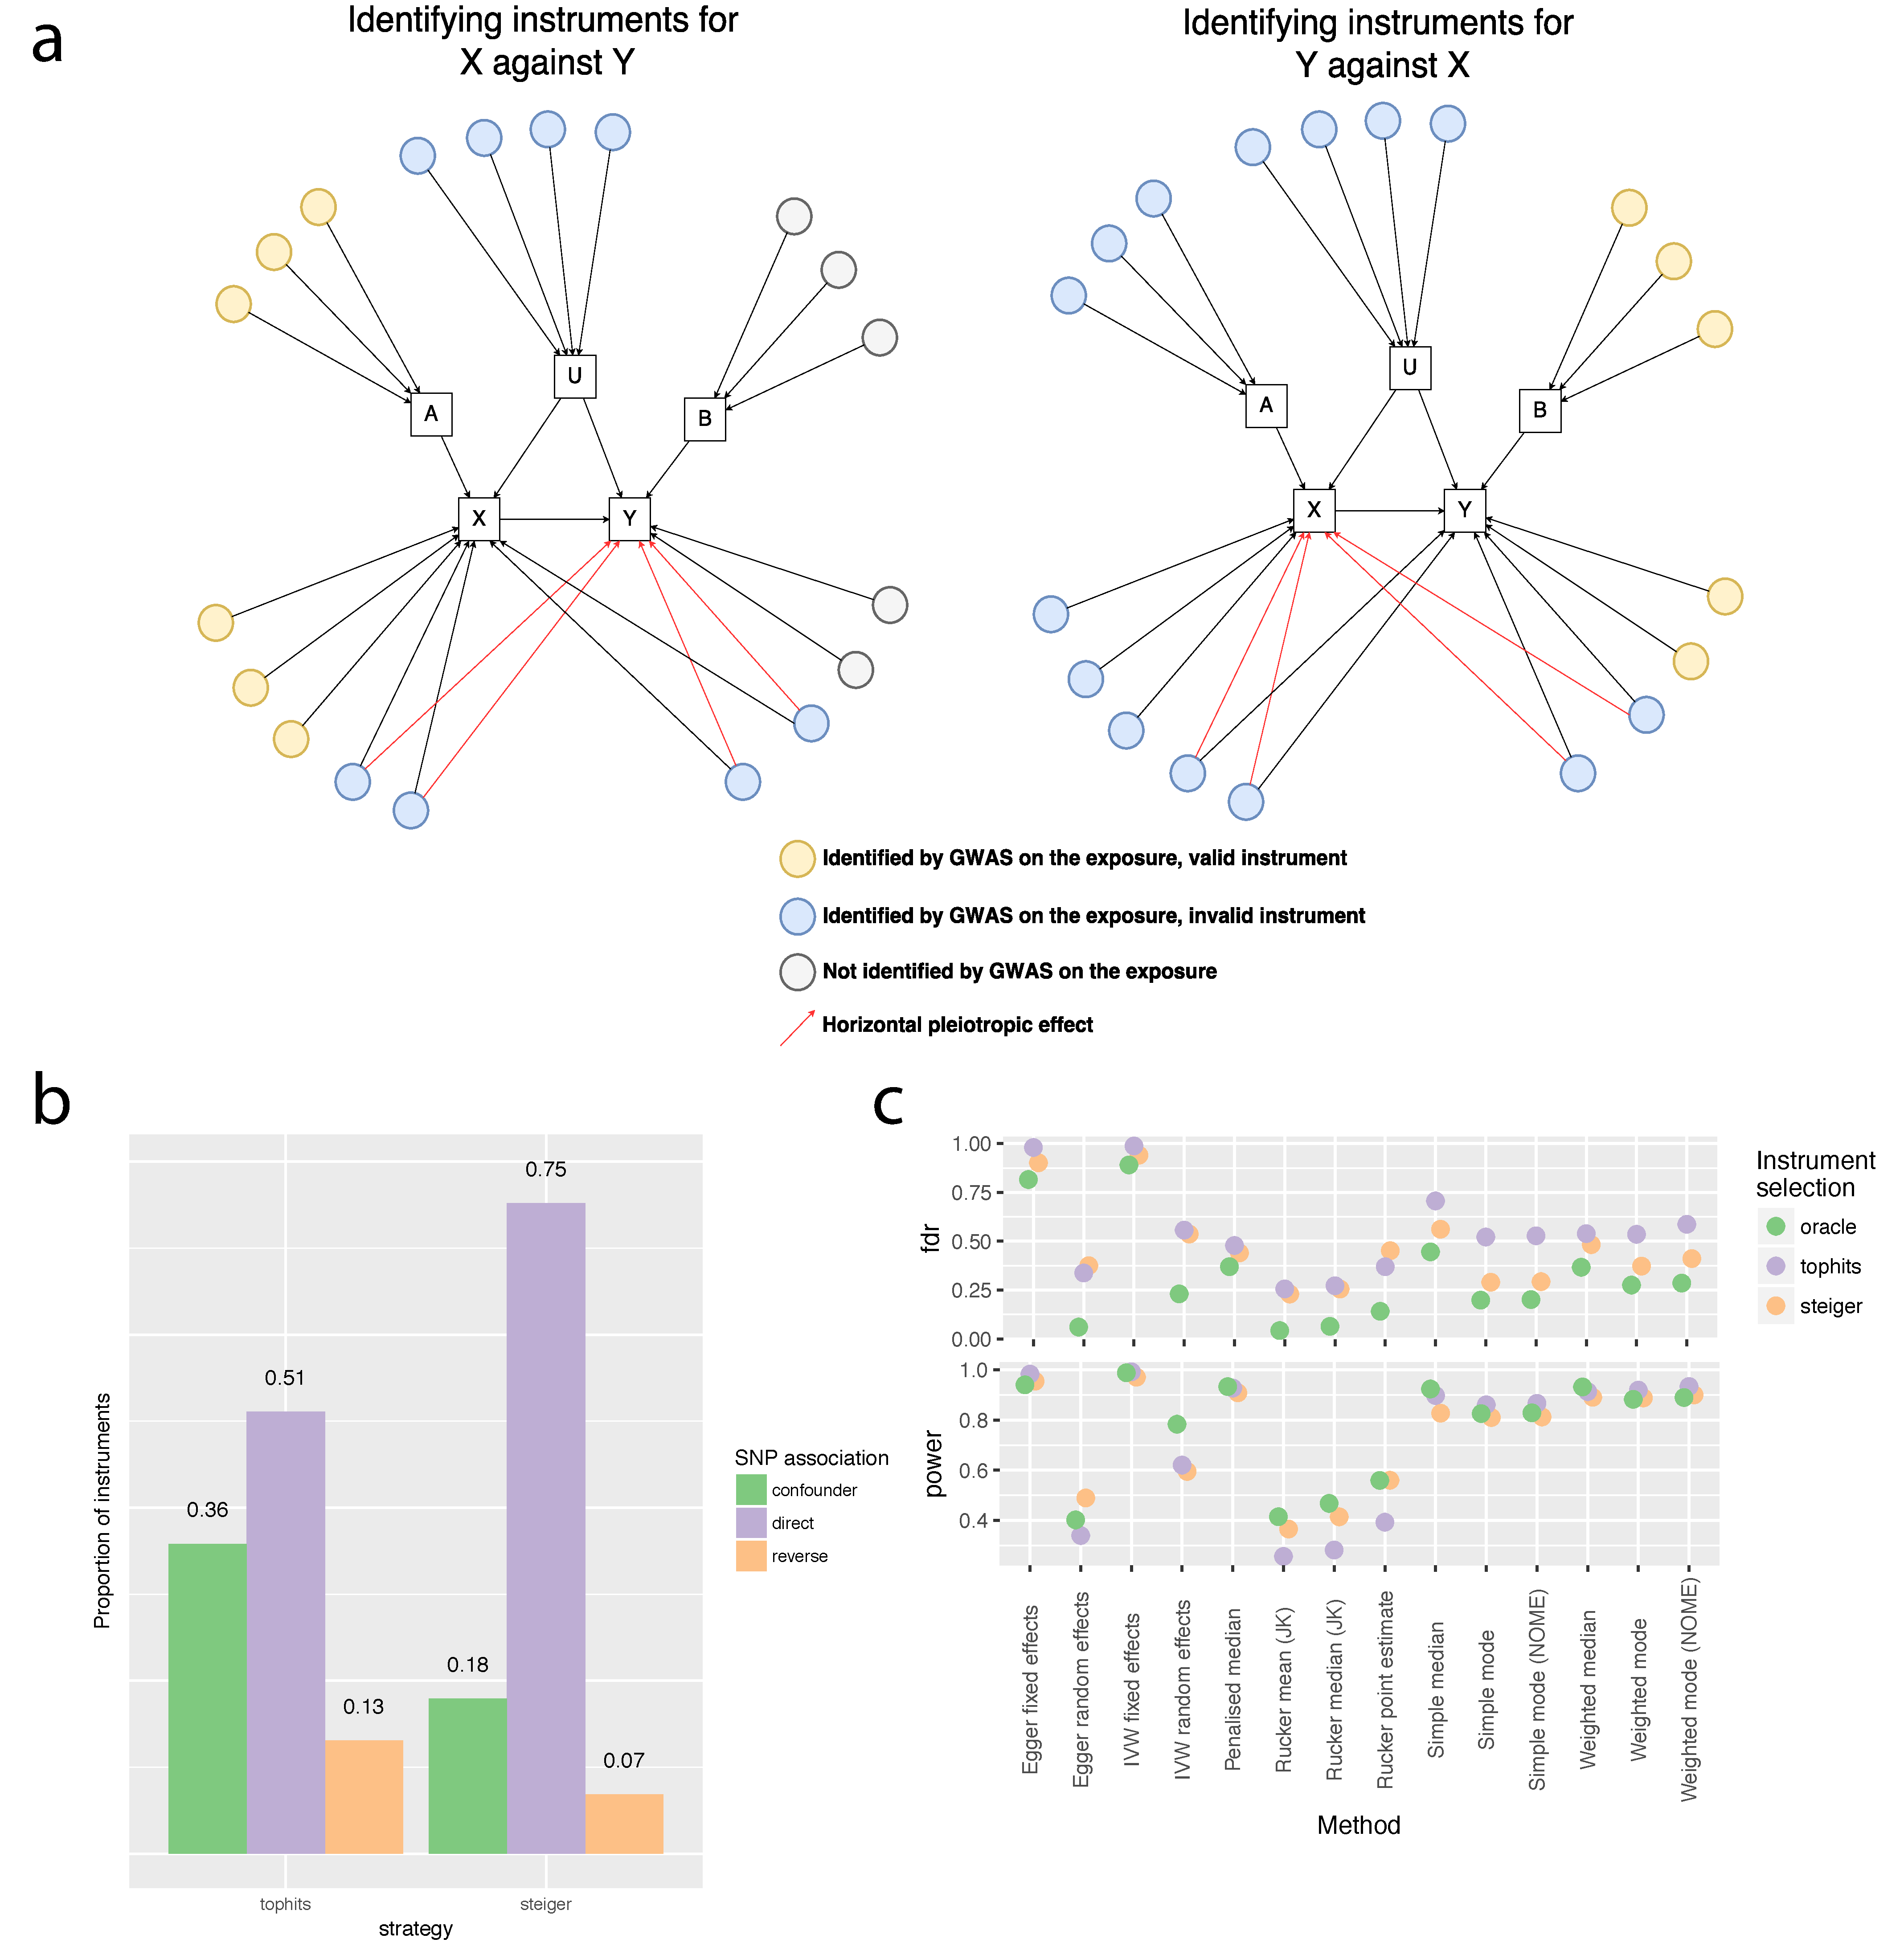
\includegraphics{images/fig1.pdf}
\caption{Simulations. a) Schematic of how GWAS with sufficient power can
lead to the selection of instrumental variables that are invalid. We
used arbitrary numbers of SNPs and confounders to simulate GWAS summary
datasets. b) Any SNP that has a direct influence on the exposure, or an
influence on a non-confounding intermediate variable, is considered a
`direct' effect. The bar-chart shows the number of direct effect
instruments retained for analysis using either the tophits approach or
the Steiger approach for instrument selection. c) Top: The false
discovery rates from null simulations for each of the 14 methods using
either tophits, Steiger filtered variants, or variants that are known to
be directly associated with the exposure (oracle, note that direct
effects can still exhibit horizontal pleiotropy in these simulations).
Bottom: The statistical power to detect true causal associations in the
non-null simulations.}
\end{figure}

\newpage

\begin{figure}
\centering
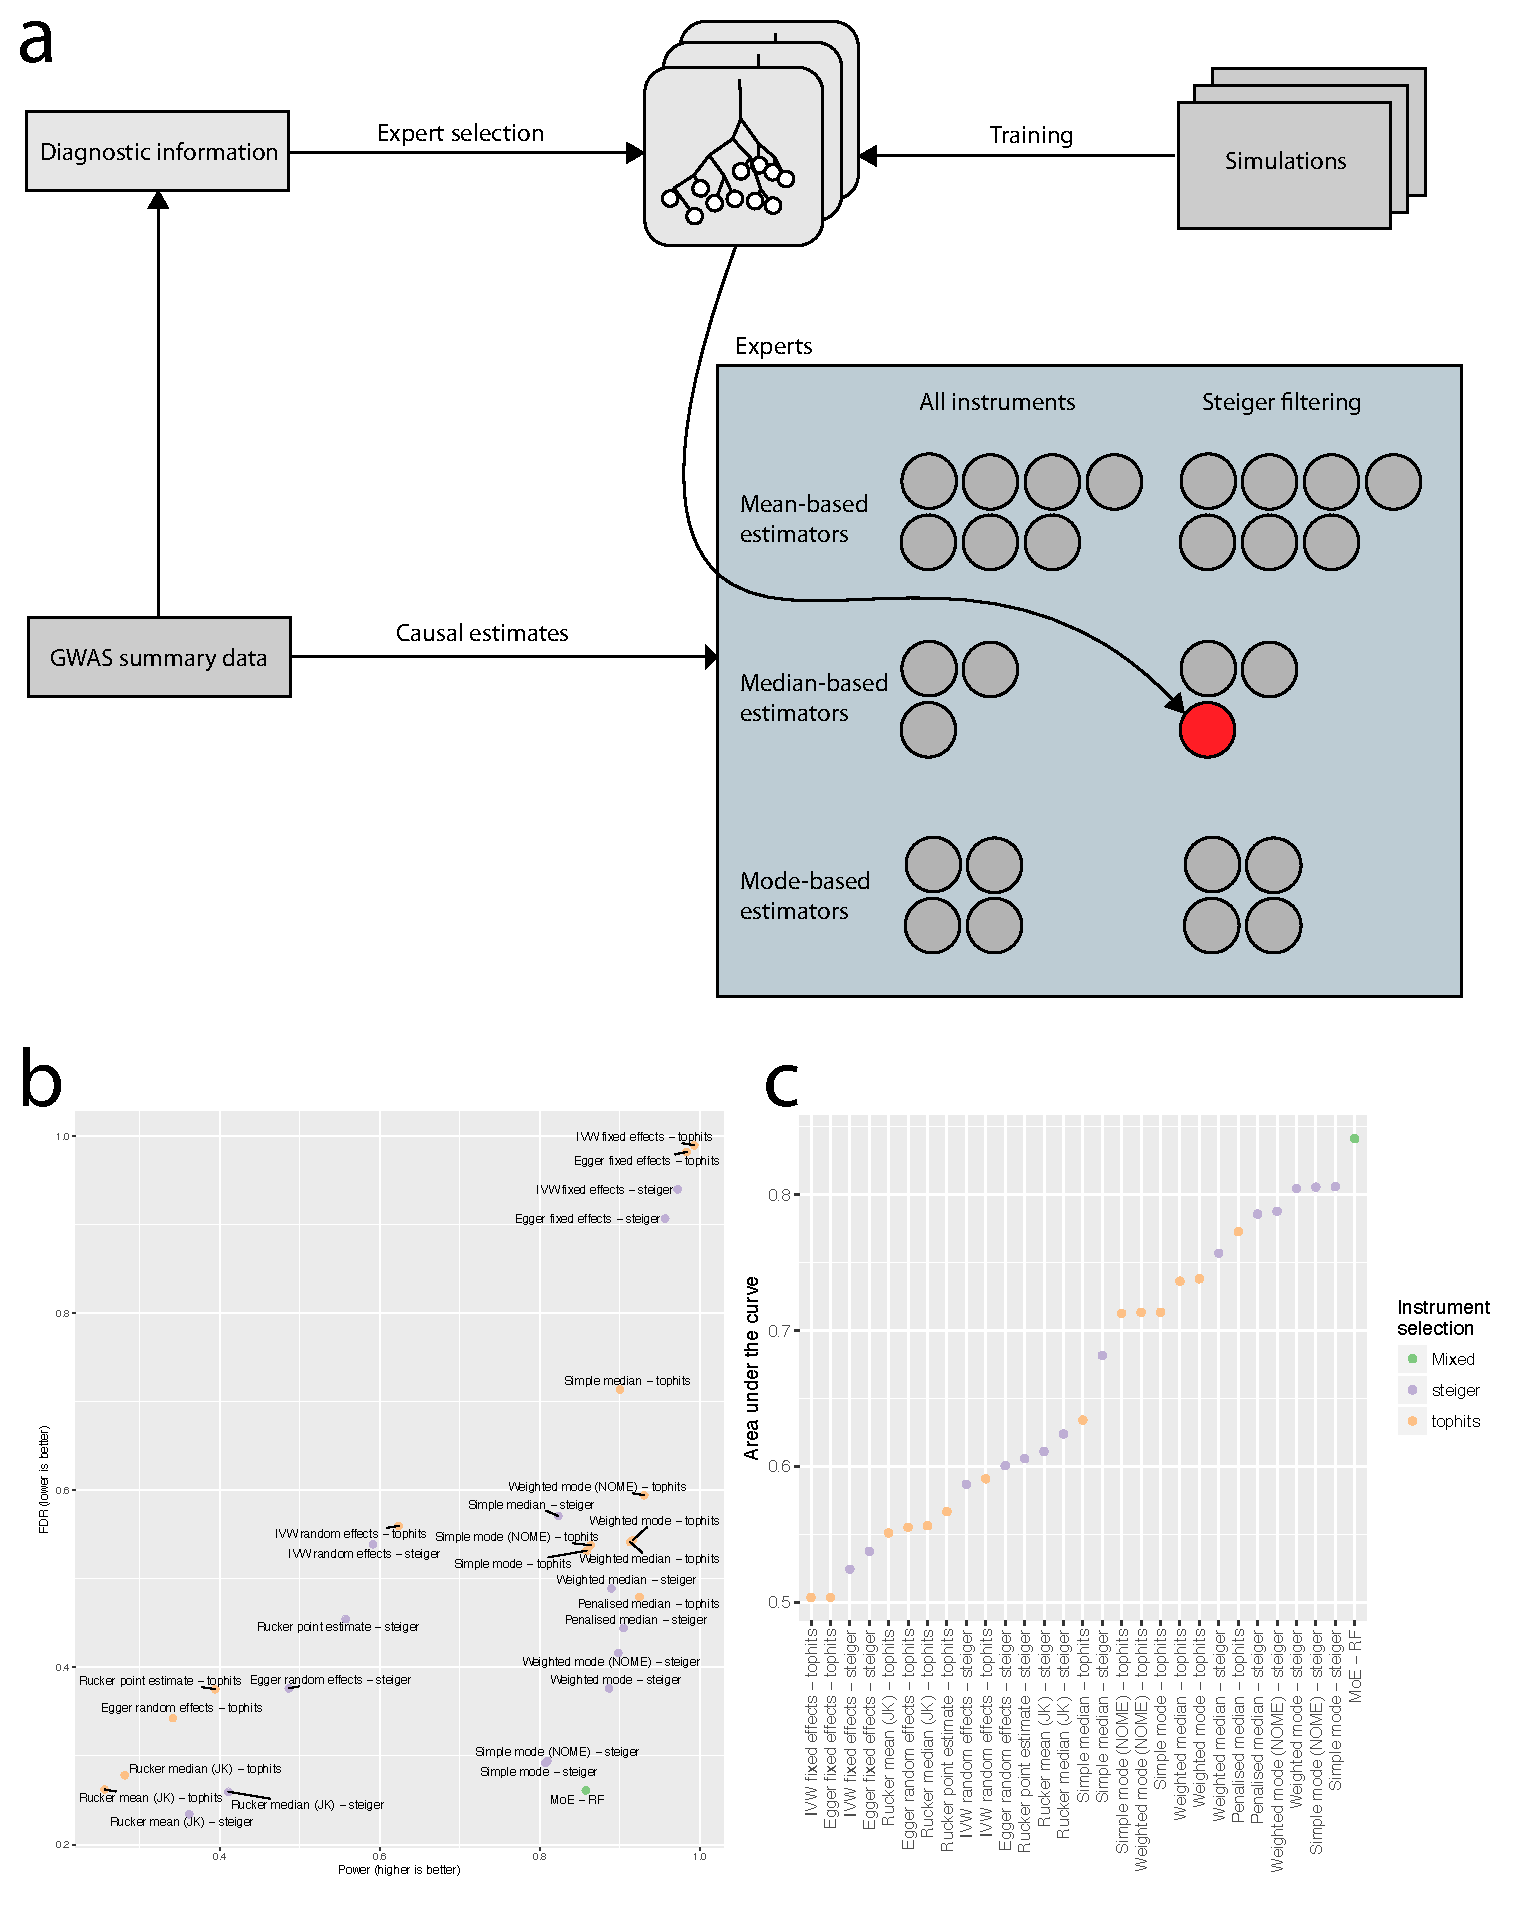
\includegraphics{images/fig2.pdf}
\caption{Mixture of experts. a) Training. Datasets are simulated that
have either null or non-null causal relationships, and MR is performed
by each of the 28 available MR methods. In the toy datasets, the columns
in black represent 53 metrics about each of the 67,000 training
simulations. The columns in red are specific to each method, they
represent how well that method performed in obtaining the correct answer
for each of the datasets. Random forests are used to learn the parameter
space of the 53 metrics in which a particular dataset is likely to
perform well. Together, this creates 28 random forest decision trees,
one for each method. b) Application. For a GWAS summary dataset, our
objective is to choose the method most likely to return the correct
causal estimate. Metrics are generated from the dataset and fed into
each of the 28 random forest decision trees. This provides us with 28
performance predictions. Finally, we use the method for which the
performance prediction is highest.}
\end{figure}

\newpage

\begin{figure}
\centering
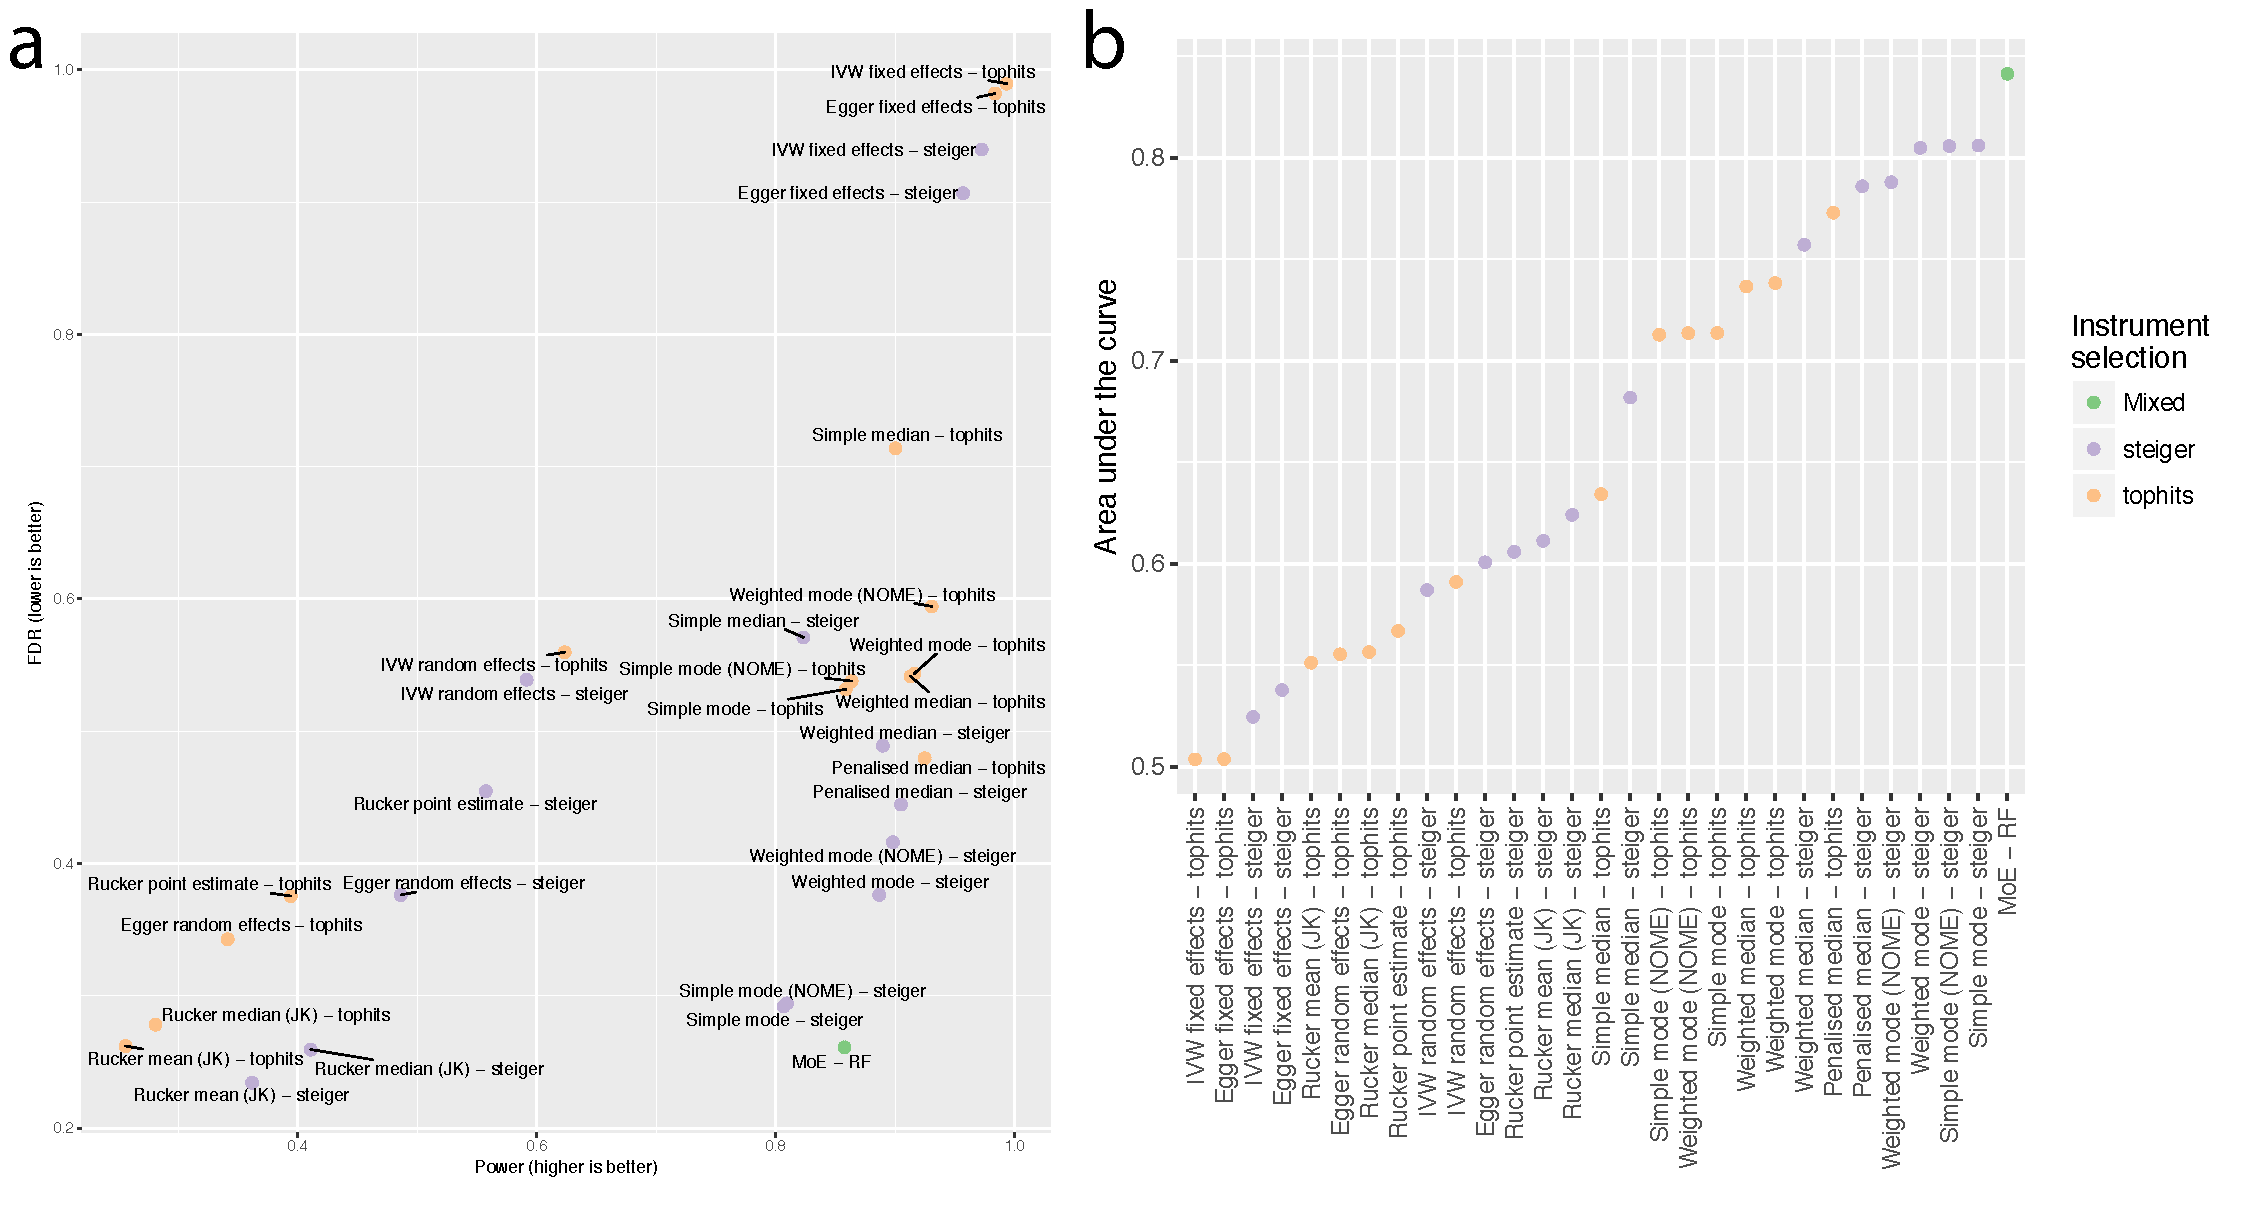
\includegraphics{images/fig3.pdf}
\caption{Performance of MoE against all other methods. a) The power for
non-null datasets is plotted against the FDR for null datasets for each
of the 28 methods, plus MoE. No single method achieved nominal FDR for
these simulations. b) Calculating the area under the ROC curve from the
values in (a) we plotted the performance in order from lowest to
highest. Under the assumption of pervasive horizontal pleiotropy, the
MoE approach is likely most effective than any other single method.}
\end{figure}

\newpage

\begin{figure}
\centering
\includegraphics{images/fig4.png}
\caption{Lookup of causal associations involving Years of Schooling. The
arrows denote causal direction and the values on the arrows denote the
causal effect estimate. Only those relationships are shown for which the
\(FDR < 0.05\).}
\end{figure}

\subsection*{References}\label{references}
\addcontentsline{toc}{subsection}{References}

\hypertarget{refs}{}
\hypertarget{ref-DaveySmith2003}{}
1. Davey Smith G, Ebrahim S. 'Mendelian randomization': can genetic
epidemiology contribute to understanding environmental determinants of
disease? International Journal of Epidemiology {[}Internet{]}. 2003
Feb;32(1):1--22. Available from:
\url{http://www.ije.oxfordjournals.org/cgi/doi/10.1093/ije/dyg070}

\hypertarget{ref-DaveySmithHemani2014}{}
2. Davey Smith G, Hemani G. Mendelian randomization: genetic anchors for
causal inference in epidemiological studies. Human molecular genetics.
2014 Jul;23(R1):R89-----R98.

\hypertarget{ref-Bowden2015}{}
3. Bowden J, Davey Smith G, Burgess S. Mendelian randomization with
invalid instruments: effect estimation and bias detection through Egger
regression. International Journal of Epidemiology. 2015;44(2):512--25.

\hypertarget{ref-Bowden2016b}{}
4. Bowden J, Davey Smith G, Haycock PC, Burgess S. Consistent Estimation
in Mendelian Randomization with Some Invalid Instruments Using a
Weighted Median Estimator. Genetic Epidemiology {[}Internet{]}. 2016
May;40(4):304--14. Available from:
\href{http://www.ncbi.nlm.nih.gov/pubmed/27061298\%20http://www.pubmedcentral.nih.gov/articlerender.fcgi?artid=PMC4849733\%20http://doi.wiley.com/10.1002/gepi.21965}{http://www.ncbi.nlm.nih.gov/pubmed/27061298 http://www.pubmedcentral.nih.gov/articlerender.fcgi?artid=PMC4849733 http://doi.wiley.com/10.1002/gepi.21965}

\hypertarget{ref-Bowden2017}{}
5. Bowden J, Del~Greco~M F, Minelli C, Davey Smith G, Sheehan N,
Thompson J. A framework for the investigation of pleiotropy in
two-sample summary data Mendelian randomization. Statistics in Medicine
{[}Internet{]}. 2017; Available from:
\url{http://doi.wiley.com/10.1002/sim.7221}

\hypertarget{ref-Hartwig2017}{}
6. Hartwig FP, Davey Smith G, Bowden J. Robust Inference In Two-Sample
Mendelian Randomisation Via The Zero Modal Pleiotropy Assumption.
bioRxiv {[}Internet{]}. 2017; Available from:
\url{http://biorxiv.org/content/early/2017/04/10/126102}

\hypertarget{ref-Hemani2017}{}
7. Hemani G, Tilling K, Davey Smith G. Orienting The Causal Relationship
Between Imprecisely Measured Traits Using Genetic Instruments. bioRxiv
{[}Internet{]}. 2017; Available from:
\url{http://biorxiv.org/content/early/2017/03/15/117101}

\hypertarget{ref-Hindorff2010}{}
8. Hindorff LA, Junkins HA, Hall PN, Mehta JP, Manolio TA. A Catalog of
Published Genome-Wide Association Studies, available at
http://www.genome.gov/gwastudies. Accessed 12/10/2010. 2010.

\hypertarget{ref-Pierce2013}{}
9. Pierce BL, Burgess S. Efficient design for Mendelian randomization
studies: subsample and 2-sample instrumental variable estimators.
American journal of epidemiology {[}Internet{]}. 2013
Oct;178(7):1177--84. Available from:
\href{http://www.pubmedcentral.nih.gov/articlerender.fcgi?artid=3783091\%7B/\&\%7Dtool=pmcentrez\%7B/\&\%7Drendertype=abstract}{http://www.pubmedcentral.nih.gov/articlerender.fcgi?artid=3783091\{\textbackslash{}\&\}tool=pmcentrez\{\textbackslash{}\&\}rendertype=abstract}

\hypertarget{ref-Hemani2016}{}
10. Hemani G, Zheng J, Wade KH, Laurin C, Elsworth B, Burgess S, et al.
MR-Base: a platform for systematic causal inference across the phenome
using billions of genetic associations. BioRxiv. 2016;10.1101/07.

\hypertarget{ref-Wagner2011}{}
11. Wagner GP, Zhang J. The pleiotropic structure of the
genotype--phenotype map: the evolvability of complex organisms. Nature
Reviews Genetics {[}Internet{]}. 2011 Mar;12(3):204--13. Available from:
\url{http://www.nature.com/doifinder/10.1038/nrg2949}

\hypertarget{ref-Hill2012a}{}
12. Hill WG, Zhang X-S. Assessing pleiotropy and its evolutionary
consequences: pleiotropy is not necessarily limited, nor need it hinder
the evolution of complexity. Nature Reviews Genetics {[}Internet{]}.
2012 Feb;13(4):296. Available from:
\url{http://www.ncbi.nlm.nih.gov/pubmed/22349131}

\hypertarget{ref-Rucker2011}{}
13. Rucker G, Schwarzer G, Carpenter JR, Binder H, Schumacher M.
Treatment-effect estimates adjusted for small-study effects via a limit
meta-analysis. Biostatistics {[}Internet{]}. 2011 Jan;12(1):122--42.
Available from:
\href{http://www.ncbi.nlm.nih.gov/pubmed/20656692\%20https://academic.oup.com/biostatistics/article-lookup/doi/10.1093/biostatistics/kxq046}{http://www.ncbi.nlm.nih.gov/pubmed/20656692 https://academic.oup.com/biostatistics/article-lookup/doi/10.1093/biostatistics/kxq046}

\hypertarget{ref-Steiger1980}{}
14. Steiger JH. Tests for comparing elements of a correlation matrix.
Psychological Bulletin. 1980;87(2):245--51.

\hypertarget{ref-Lee2013c}{}
15. Lee SH, Wray NR. Novel genetic analysis for case-control genome-wide
association studies: quantification of power and genomic prediction
accuracy. PLoS One. 2013;8(8):e71494.

\hypertarget{ref-Jordan1994}{}
16. Jordan MI, Jacobs RA. Hierarchical Mixtures of Experts and the EM
Algorithm. Neural Computation {[}Internet{]}. 1994 Mar;6(2):181--214.
Available from:
\url{http://www.mitpressjournals.org/doi/10.1162/neco.1994.6.2.181}

\hypertarget{ref-Liaw2002}{}
17. Liaw A, Wiener M. Classification and Regression by randomForest. R
News {[}Internet{]}. 2002;2(3):18--22. Available from:
\url{http://cran.r-project.org/doc/Rnews/}

\hypertarget{ref-Shin2014}{}
18. Shin S-Y, Fauman EB, Petersen A-K, Krumsiek J, Santos R, Huang J, et
al. An atlas of genetic influences on human blood metabolites. Nature
genetics {[}Internet{]}. 2014 Jun;46(6):543--50. Available from:
\url{http://dx.doi.org/10.1038/ng.2982}

\hypertarget{ref-Kettunen2016}{}
19. Kettunen J, Demirkan A, Wurtz P, Draisma HHM, Haller T, Rawal R, et
al. Genome-wide study for circulating metabolites identifies 62 loci and
reveals novel systemic effects of LPA. Nat Commun {[}Internet{]}. 2016
Mar;7. Available from:
\href{http://dx.doi.org/10.1038/ncomms11122\%20http://10.0.4.14/ncomms11122}{http://dx.doi.org/10.1038/ncomms11122 http://10.0.4.14/ncomms11122}

\hypertarget{ref-Sun2017}{}
20. Sun BB, Maranville JC, Peters JE, Stacey D, Staley JR, Blackshaw J,
et al. Consequences Of Natural Perturbations In The Human Plasma
Proteome. bioRxiv {[}Internet{]}. 2017; Available from:
\url{http://biorxiv.org/content/early/2017/05/05/134551}

\hypertarget{ref-Okbay2016}{}
21. Okbay A, Beauchamp JP, Fontana MA, Lee JJ, Pers TH, Rietveld CA, et
al. Genome-wide association study identifies 74 loci associated with
educational attainment. Nature {[}Internet{]}. 2016
May;533(7604):539--42. Available from:
\href{http://www.ncbi.nlm.nih.gov/pubmed/27225129\%20http://www.pubmedcentral.nih.gov/articlerender.fcgi?artid=PMC4883595\%20http://www.nature.com/doifinder/10.1038/nature17671}{http://www.ncbi.nlm.nih.gov/pubmed/27225129 http://www.pubmedcentral.nih.gov/articlerender.fcgi?artid=PMC4883595 http://www.nature.com/doifinder/10.1038/nature17671}

\hypertarget{ref-hemani2016mr}{}
22. Hemani G, Zheng J, Wade KH, Laurin C, Elsworth B, Burgess S, et al.
MR-Base: a platform for systematic causal inference across the phenome
using billions of genetic associations. bioRxiv. 2016;78972.

\hypertarget{ref-Zhu2016}{}
23. Zhu Z, Zhang F, Hu H, Bakshi A, Robinson MR, Powell JE, et al.
Integration of summary data from GWAS and eQTL studies predicts complex
trait gene targets. Nature Genetics {[}Internet{]}. 2016
Mar;48(5):481--7. Available from:
\url{http://www.nature.com/doifinder/10.1038/ng.3538}

\hypertarget{ref-Richardson2017}{}
24. Richardson TG, Zheng J, Davey Smith G, Timpson NJ, Gaunt TR, Relton
CL, et al. Causal epigenome-wide association study identifies CpG sites
that influence cardiovascular disease risk. bioRxiv {[}Internet{]}.
2017; Available from:
\url{http://biorxiv.org/content/early/2017/04/29/132019}

\hypertarget{ref-Noyce2017}{}
25. Noyce AJ, Kia DA, Hemani G, Nicolas A, Price TR, De Pablo-Fernandez
E, et al. Estimating the causal influence of body mass index on risk of
Parkinson disease: A Mendelian randomisation study. Brayne C, editor.
PLOS Medicine {[}Internet{]}. 2017 Jun;14(6):e1002314. Available from:
\url{http://dx.plos.org/10.1371/journal.pmed.1002314}


\end{document}
